\documentclass{article}\usepackage{graphicx, color}
%% maxwidth is the original width if it is less than linewidth
%% otherwise use linewidth (to make sure the graphics do not exceed the margin)
\makeatletter
\def\maxwidth{ %
  \ifdim\Gin@nat@width>\linewidth
    \linewidth
  \else
    \Gin@nat@width
  \fi
}
\makeatother

\IfFileExists{upquote.sty}{\usepackage{upquote}}{}
\definecolor{fgcolor}{rgb}{0.2, 0.2, 0.2}
\newcommand{\hlnumber}[1]{\textcolor[rgb]{0,0,0}{#1}}%
\newcommand{\hlfunctioncall}[1]{\textcolor[rgb]{0.501960784313725,0,0.329411764705882}{\textbf{#1}}}%
\newcommand{\hlstring}[1]{\textcolor[rgb]{0.6,0.6,1}{#1}}%
\newcommand{\hlkeyword}[1]{\textcolor[rgb]{0,0,0}{\textbf{#1}}}%
\newcommand{\hlargument}[1]{\textcolor[rgb]{0.690196078431373,0.250980392156863,0.0196078431372549}{#1}}%
\newcommand{\hlcomment}[1]{\textcolor[rgb]{0.180392156862745,0.6,0.341176470588235}{#1}}%
\newcommand{\hlroxygencomment}[1]{\textcolor[rgb]{0.43921568627451,0.47843137254902,0.701960784313725}{#1}}%
\newcommand{\hlformalargs}[1]{\textcolor[rgb]{0.690196078431373,0.250980392156863,0.0196078431372549}{#1}}%
\newcommand{\hleqformalargs}[1]{\textcolor[rgb]{0.690196078431373,0.250980392156863,0.0196078431372549}{#1}}%
\newcommand{\hlassignement}[1]{\textcolor[rgb]{0,0,0}{\textbf{#1}}}%
\newcommand{\hlpackage}[1]{\textcolor[rgb]{0.588235294117647,0.709803921568627,0.145098039215686}{#1}}%
\newcommand{\hlslot}[1]{\textit{#1}}%
\newcommand{\hlsymbol}[1]{\textcolor[rgb]{0,0,0}{#1}}%
\newcommand{\hlprompt}[1]{\textcolor[rgb]{0.2,0.2,0.2}{#1}}%

\usepackage{framed}
\makeatletter
\newenvironment{kframe}{%
 \def\at@end@of@kframe{}%
 \ifinner\ifhmode%
  \def\at@end@of@kframe{\end{minipage}}%
  \begin{minipage}{\columnwidth}%
 \fi\fi%
 \def\FrameCommand##1{\hskip\@totalleftmargin \hskip-\fboxsep
 \colorbox{shadecolor}{##1}\hskip-\fboxsep
     % There is no \\@totalrightmargin, so:
     \hskip-\linewidth \hskip-\@totalleftmargin \hskip\columnwidth}%
 \MakeFramed {\advance\hsize-\width
   \@totalleftmargin\z@ \linewidth\hsize
   \@setminipage}}%
 {\par\unskip\endMakeFramed%
 \at@end@of@kframe}
\makeatother

\definecolor{shadecolor}{rgb}{.97, .97, .97}
\definecolor{messagecolor}{rgb}{0, 0, 0}
\definecolor{warningcolor}{rgb}{1, 0, 1}
\definecolor{errorcolor}{rgb}{1, 0, 0}
\newenvironment{knitrout}{}{} % an empty environment to be redefined in TeX

\usepackage{alltt}
\usepackage{amsmath, amsthm, parskip, graphicx}

\frenchspacing







\title{Informal explination of study ``Ecotype detection in (geometric) morphometric data''}
\author{Peter D Smits \and Benjamin Frable}

\begin{document}
\maketitle

\section{Introduction}
Stuff

\section{Materials and Methods}

\subsection{Fish}
Four families of Characiformes: Anostomidae, Chilodontidae, Curimatidae, and Prochilodontidae.

Total 78 specimens for four families of Characiformes: 18 Anostomidae, 4 Chilodontidae, 48 Curimatidae, and 8 Prochilodontidae.

\subsection{Morphometric analysis}
35 two-dimensional landmarks and the head and neck. Landmarks were selected for some reason and were collected using TPSDig2. Generalized Procrustes analysis was used to remove the effects of orientation, rotation, and scaling CITATION. Following this, points were projected onto tangent space using principal components analysis CITATION. This was done in the R statistical programming language CITATION using the ``shapes'' CITATION and ``geomorph'' packages.

\subsection{Machine learning}
The predictive accuracy of shape for family as assessed using multinomial logistic regression and a training set of 75\% of all samples and a test set of 25\% of all samples. Multinomial logist regression is a generalization of the standard logistic regression where instead of a binary response variable, there are multiple categorical responses. In this case, the multinomial response variable was family while predictors were the pricipal components of shape.

Pricipal components analysis produced 70 eigenscores for every taxa and there are only 78 taxa sampled, it is necessary to select only from a subset of the possible predictors. Models were compared using the second-order Akaike's information criterion (AICc) where lower values indicate a better bias-variance trade off between the number of predictors and the likelihood of the model CITATIONS while taking into account sample size. 

Model selection is not without uncertainty, as some models may have very close AICc values. Model selection was done using \(\delta\)AICc and Akaike weight values CITATION. \(\delta\)AICc values are calculated as the difference between the AICc of a model and the AICc of the AICc-best model, or the model with the lowest AICc. Akaike weights sum to 1 and represent the propotional amount of information explained by a particular model and are approximately the model selection probability. Models with a \(\delta\)AICc of less than 2 were considered approximately identical in information to the AICc best model, while models with a \(\delta\)AICc of less than 6 were considered as plausible but suboptimal. Models with a \(\delta\)AICc of greater than 10 were considered extremely poor.

I will eventually be making predictions from a model using averaged parameters of the first 95\% confidence set of models, as measured by Akaike weights CITATION.

The models compared varied between 1 and 7 pricipal component predictors, producing models with 6, 9, 12, 15, 18, 21, 24 parameters respectively. 

I did some model training using ``caret'' and ``e1071'' packages. Need to explain.

Following model training and model comparison, the AICc-best model was used to predict the family of the testing data set described above.

\section{Results}

\subsection{Morphometric analysis}



\begin{figure}[p]
  \centering
  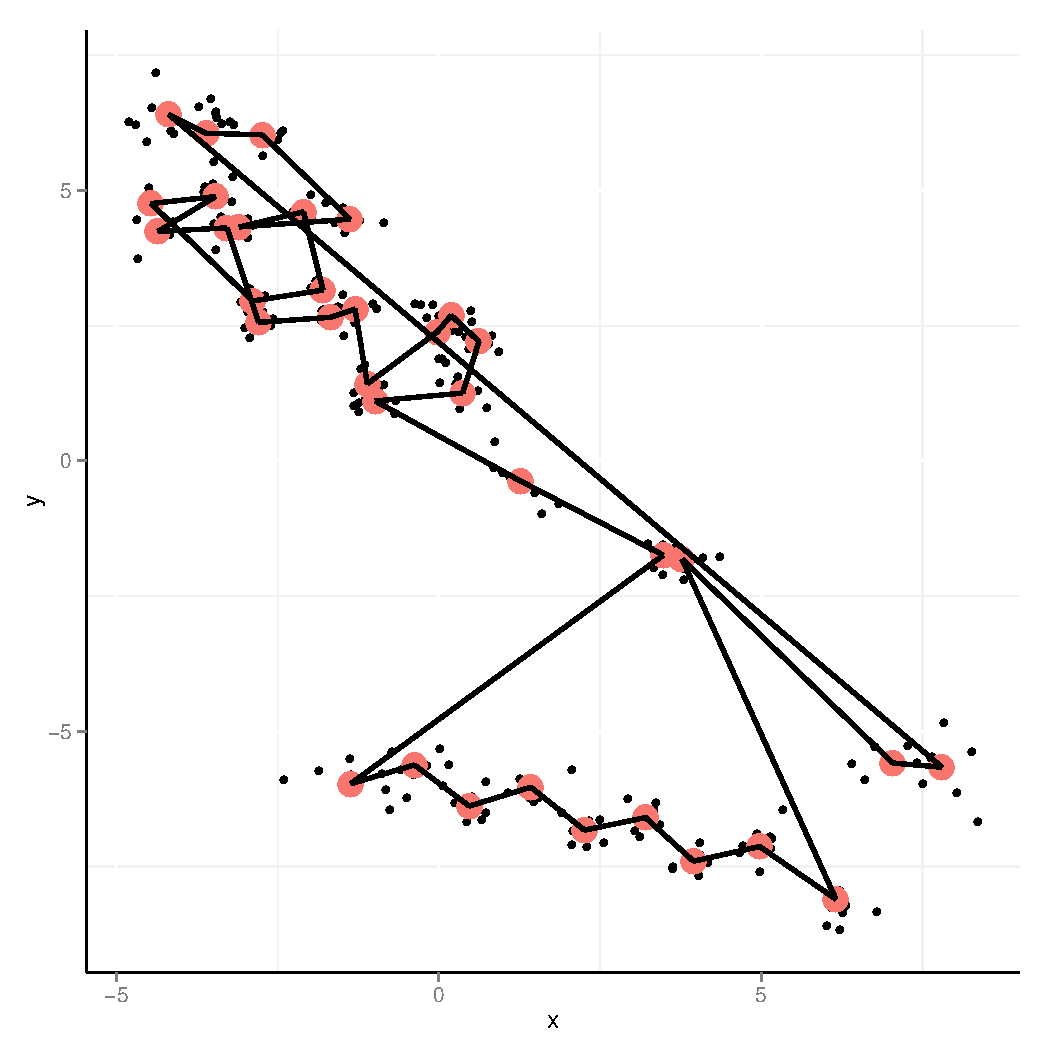
\includegraphics[height = 0.4\textheight, keepaspectratio = true]{figure/pls-fits3}
  \caption{Procrustes fit landmark dispersion for all taxa in comparison to mean landmark position in red.}
  \label{fig:fish-fit}
\end{figure}

\begin{knitrout}
\definecolor{shadecolor}{rgb}{1, 1, 1}\color{fgcolor}
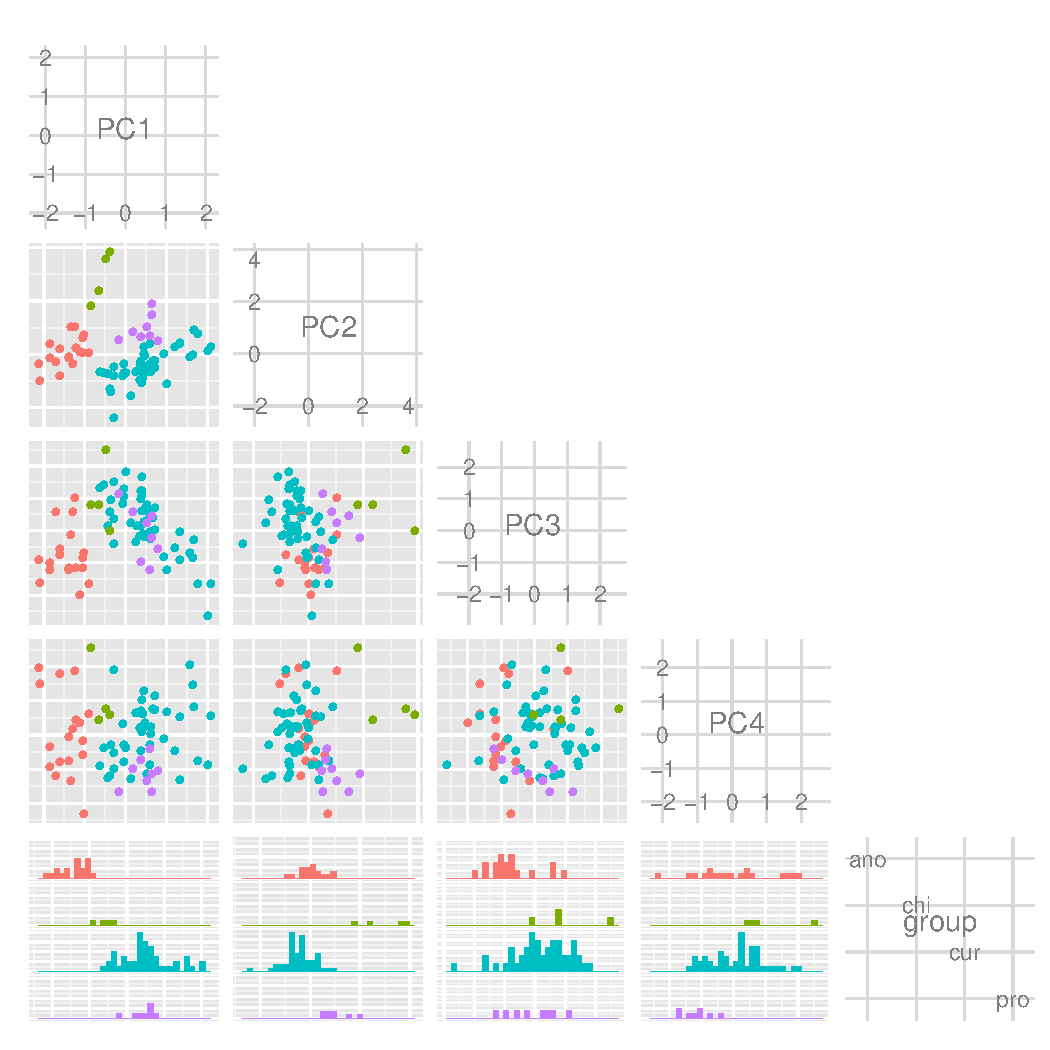
\includegraphics[width=\maxwidth]{figure/pca-plots} 

\end{knitrout}

\begin{figure}[p]
  \centering
  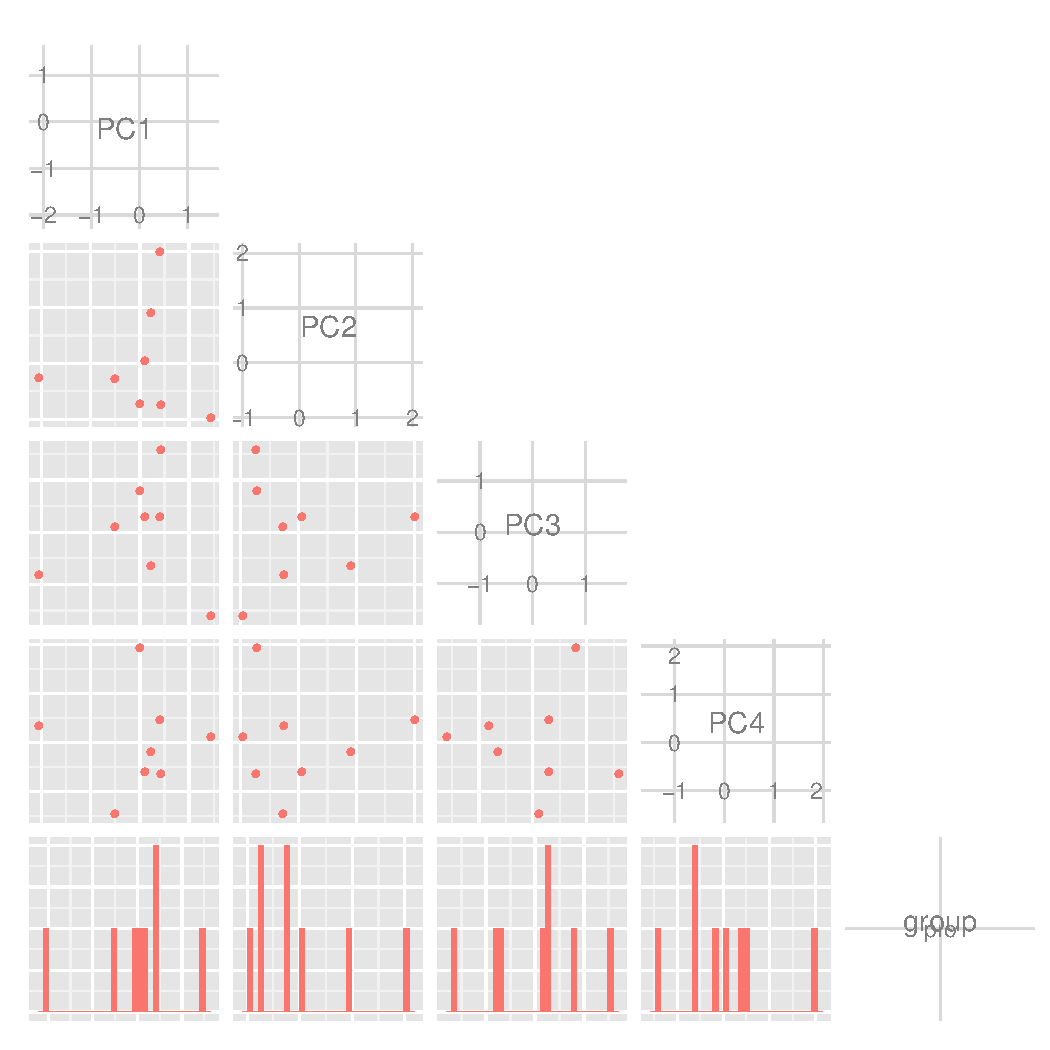
\includegraphics[height = 0.4\textheight, keepaspectratio = true]{figure/pca-plots3}
  \caption{Comparison of first four pricipal components of Procrustes fit landmarks. Familes are highlighted.}
  \label{fig:fish-pca}
\end{figure}

\subsection{Machine learning}

% model selection table
% latex table generated in R 2.15.2 by xtable 1.7-0 package
% Fri Jan 11 16:26:20 2013
\begin{table}[p]
\begin{center}
\begin{tabular}{rlllllllllrrrrr}
  \hline
 & (Intercept) & PC1 & PC2 & PC3 & PC4 & PC5 & PC6 & PC7 & family & df & logLik & AICc & delta & weight \\ 
  \hline
2 & + & + & + &  &  &  &  &  &  & 9.00 & -14.34 & 50.35 & 0.00 & 0.97 \\ 
  3 & + & + & + & + &  &  &  &  &  & 12.00 & -13.18 & 57.15 & 6.80 & 0.03 \\ 
  4 & + & + & + & + & + &  &  &  &  & 15.00 & -11.46 & 64.09 & 13.74 & 0.00 \\ 
  5 & + & + & + & + & + & + &  &  &  & 18.00 & -8.82 & 70.73 & 20.39 & 0.00 \\ 
  1 & + & + &  &  &  &  &  &  &  & 6.00 & -33.71 & 81.03 & 30.68 & 0.00 \\ 
  6 & + & + & + & + & + & + & + &  &  & 21.00 & -7.10 & 81.17 & 30.82 & 0.00 \\ 
  7 & + & + & + & + & + & + & + & + &  & 24.00 & -0.04 & 83.38 & 33.04 & 0.00 \\ 
   \hline
\end{tabular}
\caption{Model selection table.}
\label{tab:fish-tab}
\end{center}
\end{table}



% latex table generated in R 2.15.2 by xtable 1.7-0 package
% Fri Jan 11 16:26:20 2013
\begin{table}[p]
\begin{center}
\begin{tabular}{rrrrr}
  \hline
 & ano & chi & cur & pro \\ 
  \hline
ano &   4 &   0 &   0 &   0 \\ 
  chi &   0 &   1 &   0 &   0 \\ 
  cur &   0 &   0 &  12 &   0 \\ 
  pro &   0 &   0 &   0 &   2 \\ 
   \hline
\end{tabular}
\caption{Confusion matrix.}
\label{tab:fish-mod}
\end{center}
\end{table}





\begin{figure}[p]
  \centering
  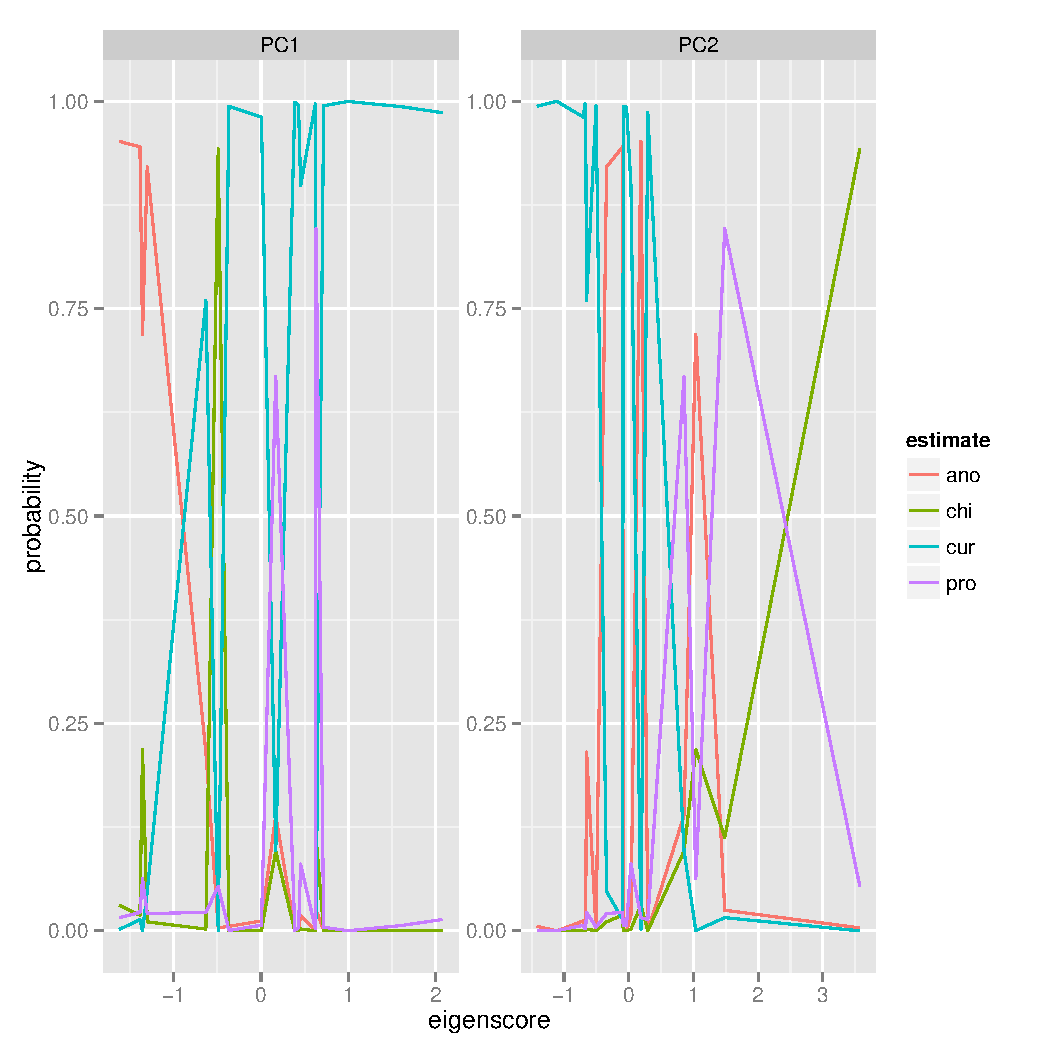
\includegraphics[width = 0.4\textwidth, keepaspectratio = true]{figure/logistic-plots}
  \caption{Relative probabilities of Characiform family identification from the first two principal components of shape. The first two pricipal components are plotted here because they are the predictors of family from the AICc-best model.}
  \label{fig:fish-logistic}
\end{figure}


\section{Discussion}


\end{document}
